In this chapter, we will now extend our study on composite resonator systems. Such as, we will increase the number of resonators in our system. These structures, that will be discussed here, were not optimized to achieve enhanced dispersion. Rather the purpose of these analyses is to demonstrate the versatility and distinct optical characteristics of cascaded resonances which are obtained by cascading three resonators (Fig. 4.1). For the scope of this thesis, the system will consist of ring-shaped resonators and thus we will study properties of such ring resonators and their mutual coupling effects.
\section{Triple Ring Resonator System}
Now we introduce a new resonator geometry. Basically, we are to simply add another ring above the coupled two resonator system which was discussed in greater detail Chapter 3. Now we have a three-resonator system with each having their own distinct resonant frequencies. These resonators show distinct properties due to the introduction of an additional ring with a higher Quality-factor, coupled to the two resonator system. This allows us to observe multiple resonances and observe phenomenons like CRIT and CRIA with another perspective. This also enables us to simultaneously measure these effects in a single system and thus obtain versatile transmission and dispersion.

The illustration in Fig. 4.1 shows us that the three rings are mutually coupled to each other and only the first ring is coupled to the optical waveguide. The incident energy from the input is labeled as $E_{1}$ which couples to the first resonator due to evanescent coupling. The energy is then transferred to $E_{3}$. This energy travels the first ring and is again coupled into the  as $E_{5}$ and then again into the third resonator with energy $E_{7}$. Then it loops back into the waveguide as $E_{8}$, $E_{6}$ and $E_{4}$ respectively to couple back to the waveguide, each acquiring a distinct phase shift and outputs the signal with energy $E_{2}$. Here, $E_{3}$ and $E_{4}$ describes the circulating fields of the first resonator. Evanescent coupling between the first and the second resonator results in the circulating fields of the resonator two labeled $E_{5}$ and $E_{6}$. A similar mechanism leads to the excitation of the resonant mode of the third cavity, with circulating fields described by $E_{7}$ and $E_{8}$.

\begin{figure}[h]
\centering
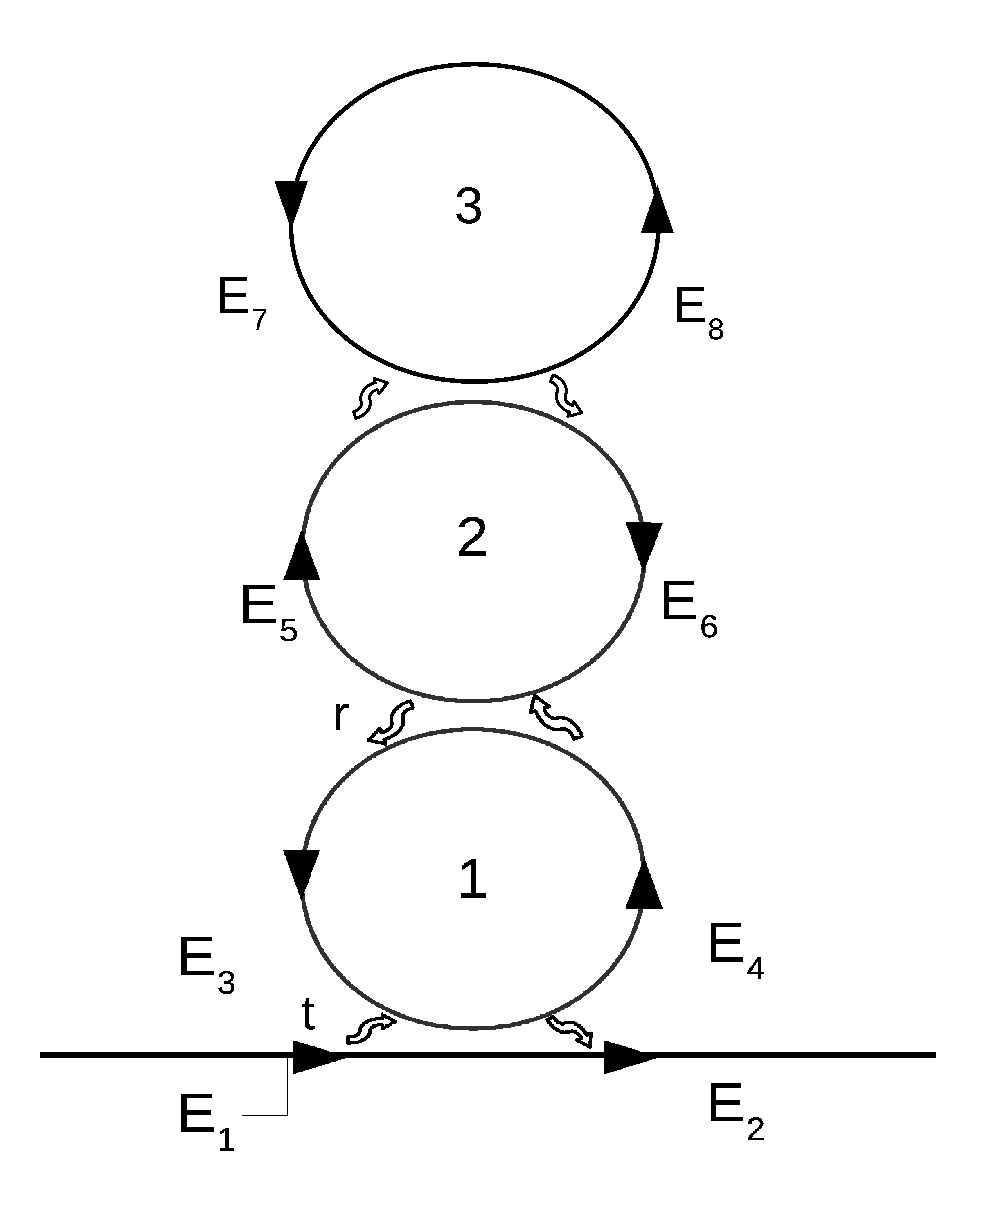
\includegraphics[scale=0.45]{triple_ring_resonator.eps}
\caption{Basic illustration of three ring resonator geometery along with its respective fields. Here, first resonator is labeled as 1, second is labeled as 2, and third is labeled as 3.}
\end{figure}

\subsection{Transmission and Phase relations}
The complex transmitivity and its respective phase can be determined by equations 4.1 and 4.2 respectively. 

\begin{equation}
\frac{E_{t}}{E_{i}} = \frac{r_{1} - a_{1} \, r_{12} \, e^{i\phi_{1}}}{1 - r_{1}\, r_{12}\, a_{1}\, e^{i\phi_{1}}}
\end{equation}

where, 
\begin{align*}
r_{12} = \frac{r_{2} - a_{2}\, r_{23}\, e^{i \phi_{2}}} {1 - r_{2} r_{23}\, a_{2}\, e^{i \phi_{2}}} 
\end{align*}
and,
\begin{align*}
r_{23} = \frac{r_{3} - a_{3}\, e^{i \phi_{3}}} {1 - r_{3}\, a_{3}\, e^{i \phi_{3}}} 
\end{align*}

Similarly, the effective phase of the complex transmitivity is given by:

\begin{equation}
\phi_{eff} = \arctan[{\frac{r_{1} |r_{12}| a_{1} \sin{(\phi_{1} + \phi_{12})}}{1 - |r_{12}| a_{1} \cos{(\phi_{1} + \phi_{12})}}}] - \arctan[{\frac{|r_{12}| a_{1} \sin{(\phi_{1} + \phi_{12})}}{r_{1} - |r_{12}| a_{1} \cos{(\phi_{1} + \phi_{12})}}}]
\end{equation}

Now we use these equations to observe characteristics of triple cavity resonances.

\section{Passive Three Resonator Results}
We can obtain very interesting results from a passive three resonator systems some of which are discussed in this section. Fig. 4.2 displays CRIT inside a CRIA resonance hence negative group index and fast light are obtained on resonant frequencies while large values of subluminal group indexes are clearly apparent at the off-resonance transmission. When resonator two is allowed to couple with the third resonator, due to its effects there is an on-resonance peak inside the CRIA dip. These cascaded resonances can help play an important role in the tunability of fast and slow light and/or in large and small absorption of resonant frequencies. This may lead to new applications in communication technology and related fields. These kinds of effects which were observed in atomic systems had shortcomings due to a large amount of absorption and had low-temperature maintenance problems. Now, these effects can be observed in photonic resonators which are operatable at room temperatures.
\subsection{CRIT inside CRIA}
In Fig. 4.2, we see that the transmission spectrum looks like a CRIA dip, meaning it will display the properties of CRIA. The system parameters are given as, $r_{1} = 0.898945$, $r_{2} = 0.999958$, and $r_{3} = 0.999999$. The $\mathcal{Q}-factors$ are $1\times10^{5}, 1\times10^{6}$ and $1\times10^{7}$ for first second and third resonator respectively. When we zoom into the graph (as shown on the right), we observe that there is another peak rising within the CRIA, showing the feature due to the resonance of the third resonator. Thus now we have CRIT inside a CRIA transmission. This will allow us to have transmission intensity larger while maintaining the characteristics of CRIA dispersion. Now we can have more light in CRIA mediate transmission. This means we can have fast light dispersion on on-resonant frequencies, which can be enhanced by adjusting mutual coupling of the resonators.

The effective phase of the system is shown in red where we see the curve similar to a single resonator. But when we zoom into the middle of the curve, we see features inside which characterize the presence of three cavities. The zoomed version is shown on the right in Fig. 4.2 and it displays a sharp negative slope on resonance leading to a group index value of $\approx -214016$. Thus the light we are receiving in the transmission has a negative group velocity i.e. fast light and we conclude that we have superluminal light along with large transmission owing to cascaded CRIT and CRIA.

\begin{figure}[t]
\centering
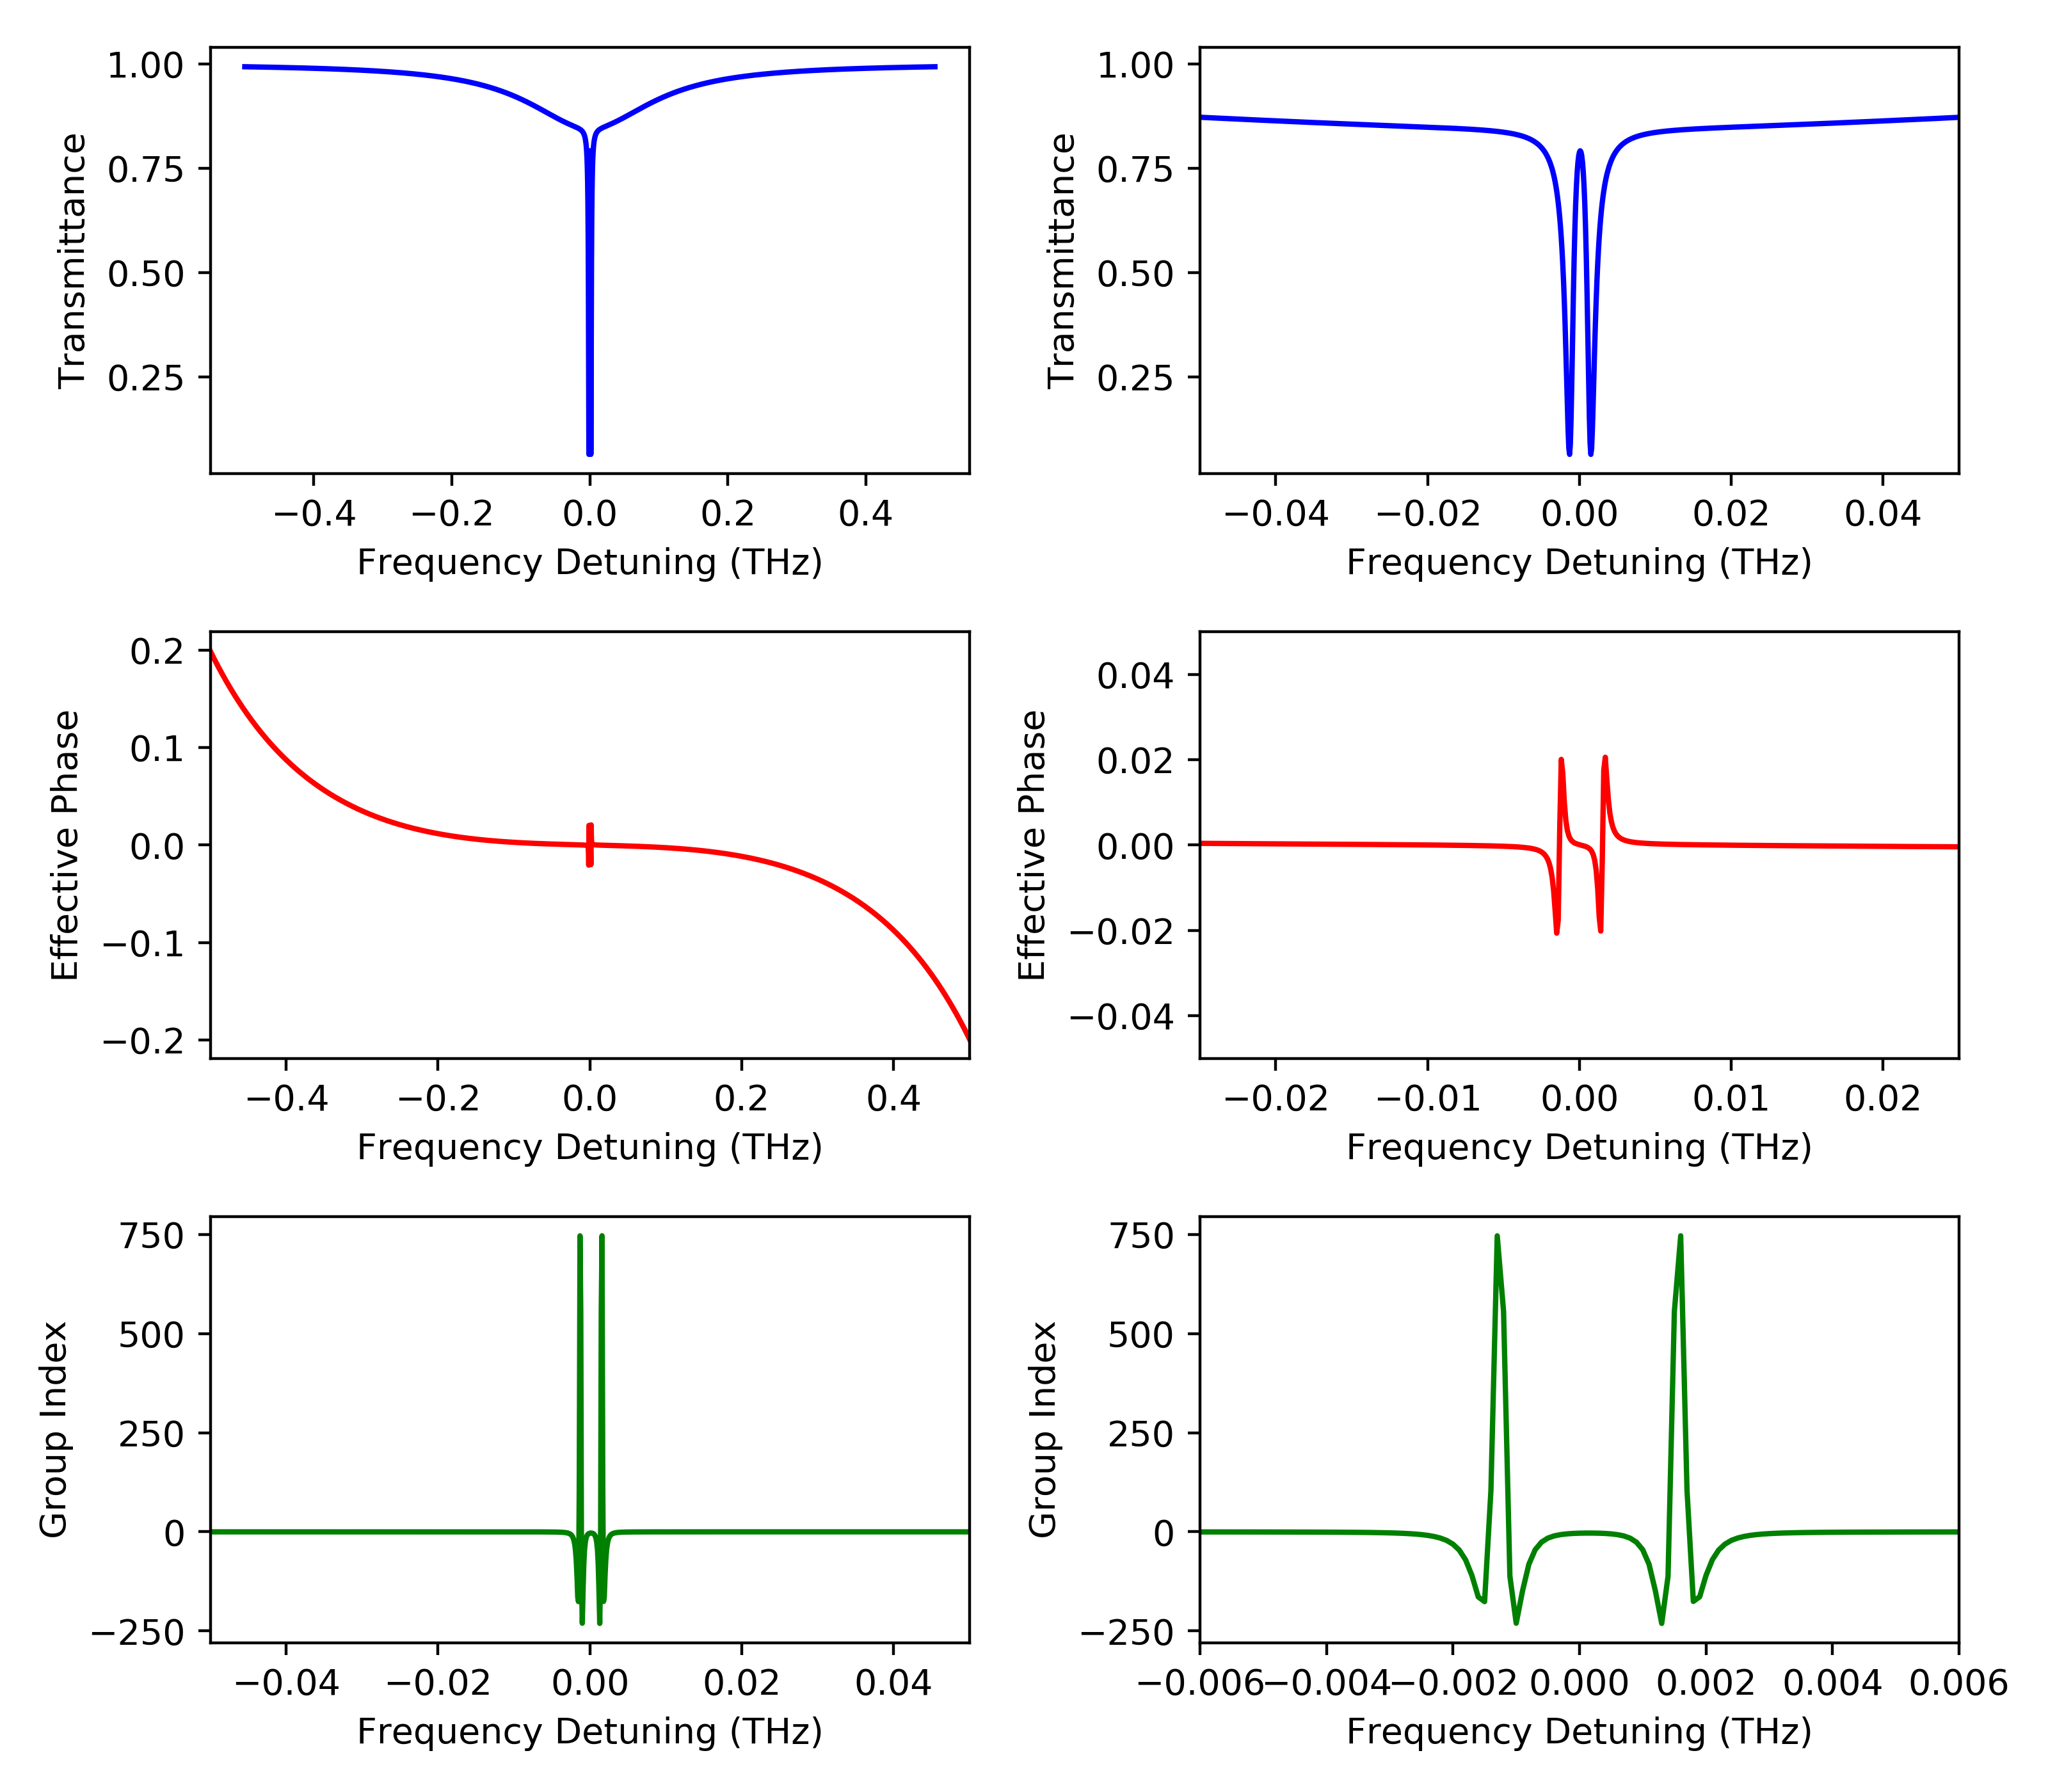
\includegraphics[width=1\textwidth]{EIT_EIA_all.png}
\caption{CRIT observered in an CRIA transmission in three resonator system with its phase in red and group index in green.}
\end{figure}

\newpage
\subsection{CRIA inside CRIT}

After these interesting results, let us now move towards another useful transmission spectrum of our triple resonator system (see Fig. 4.3). The system parameters are given as, $r_{1} = 0.987655$, $r_{2} = 0.999888$, and $r_{3} = 0.999989$. The $\mathcal{Q}-factors$ are $1\times10^{5}, 1\times10^{6}$ and $1\times10^{7}$ for first second and third resonator respectively. This spectrum is also achieved by the same arrangement of the resonators and now we have changed the couplings once more to obtain an interesting result. 

\begin{figure}[t]
\centering
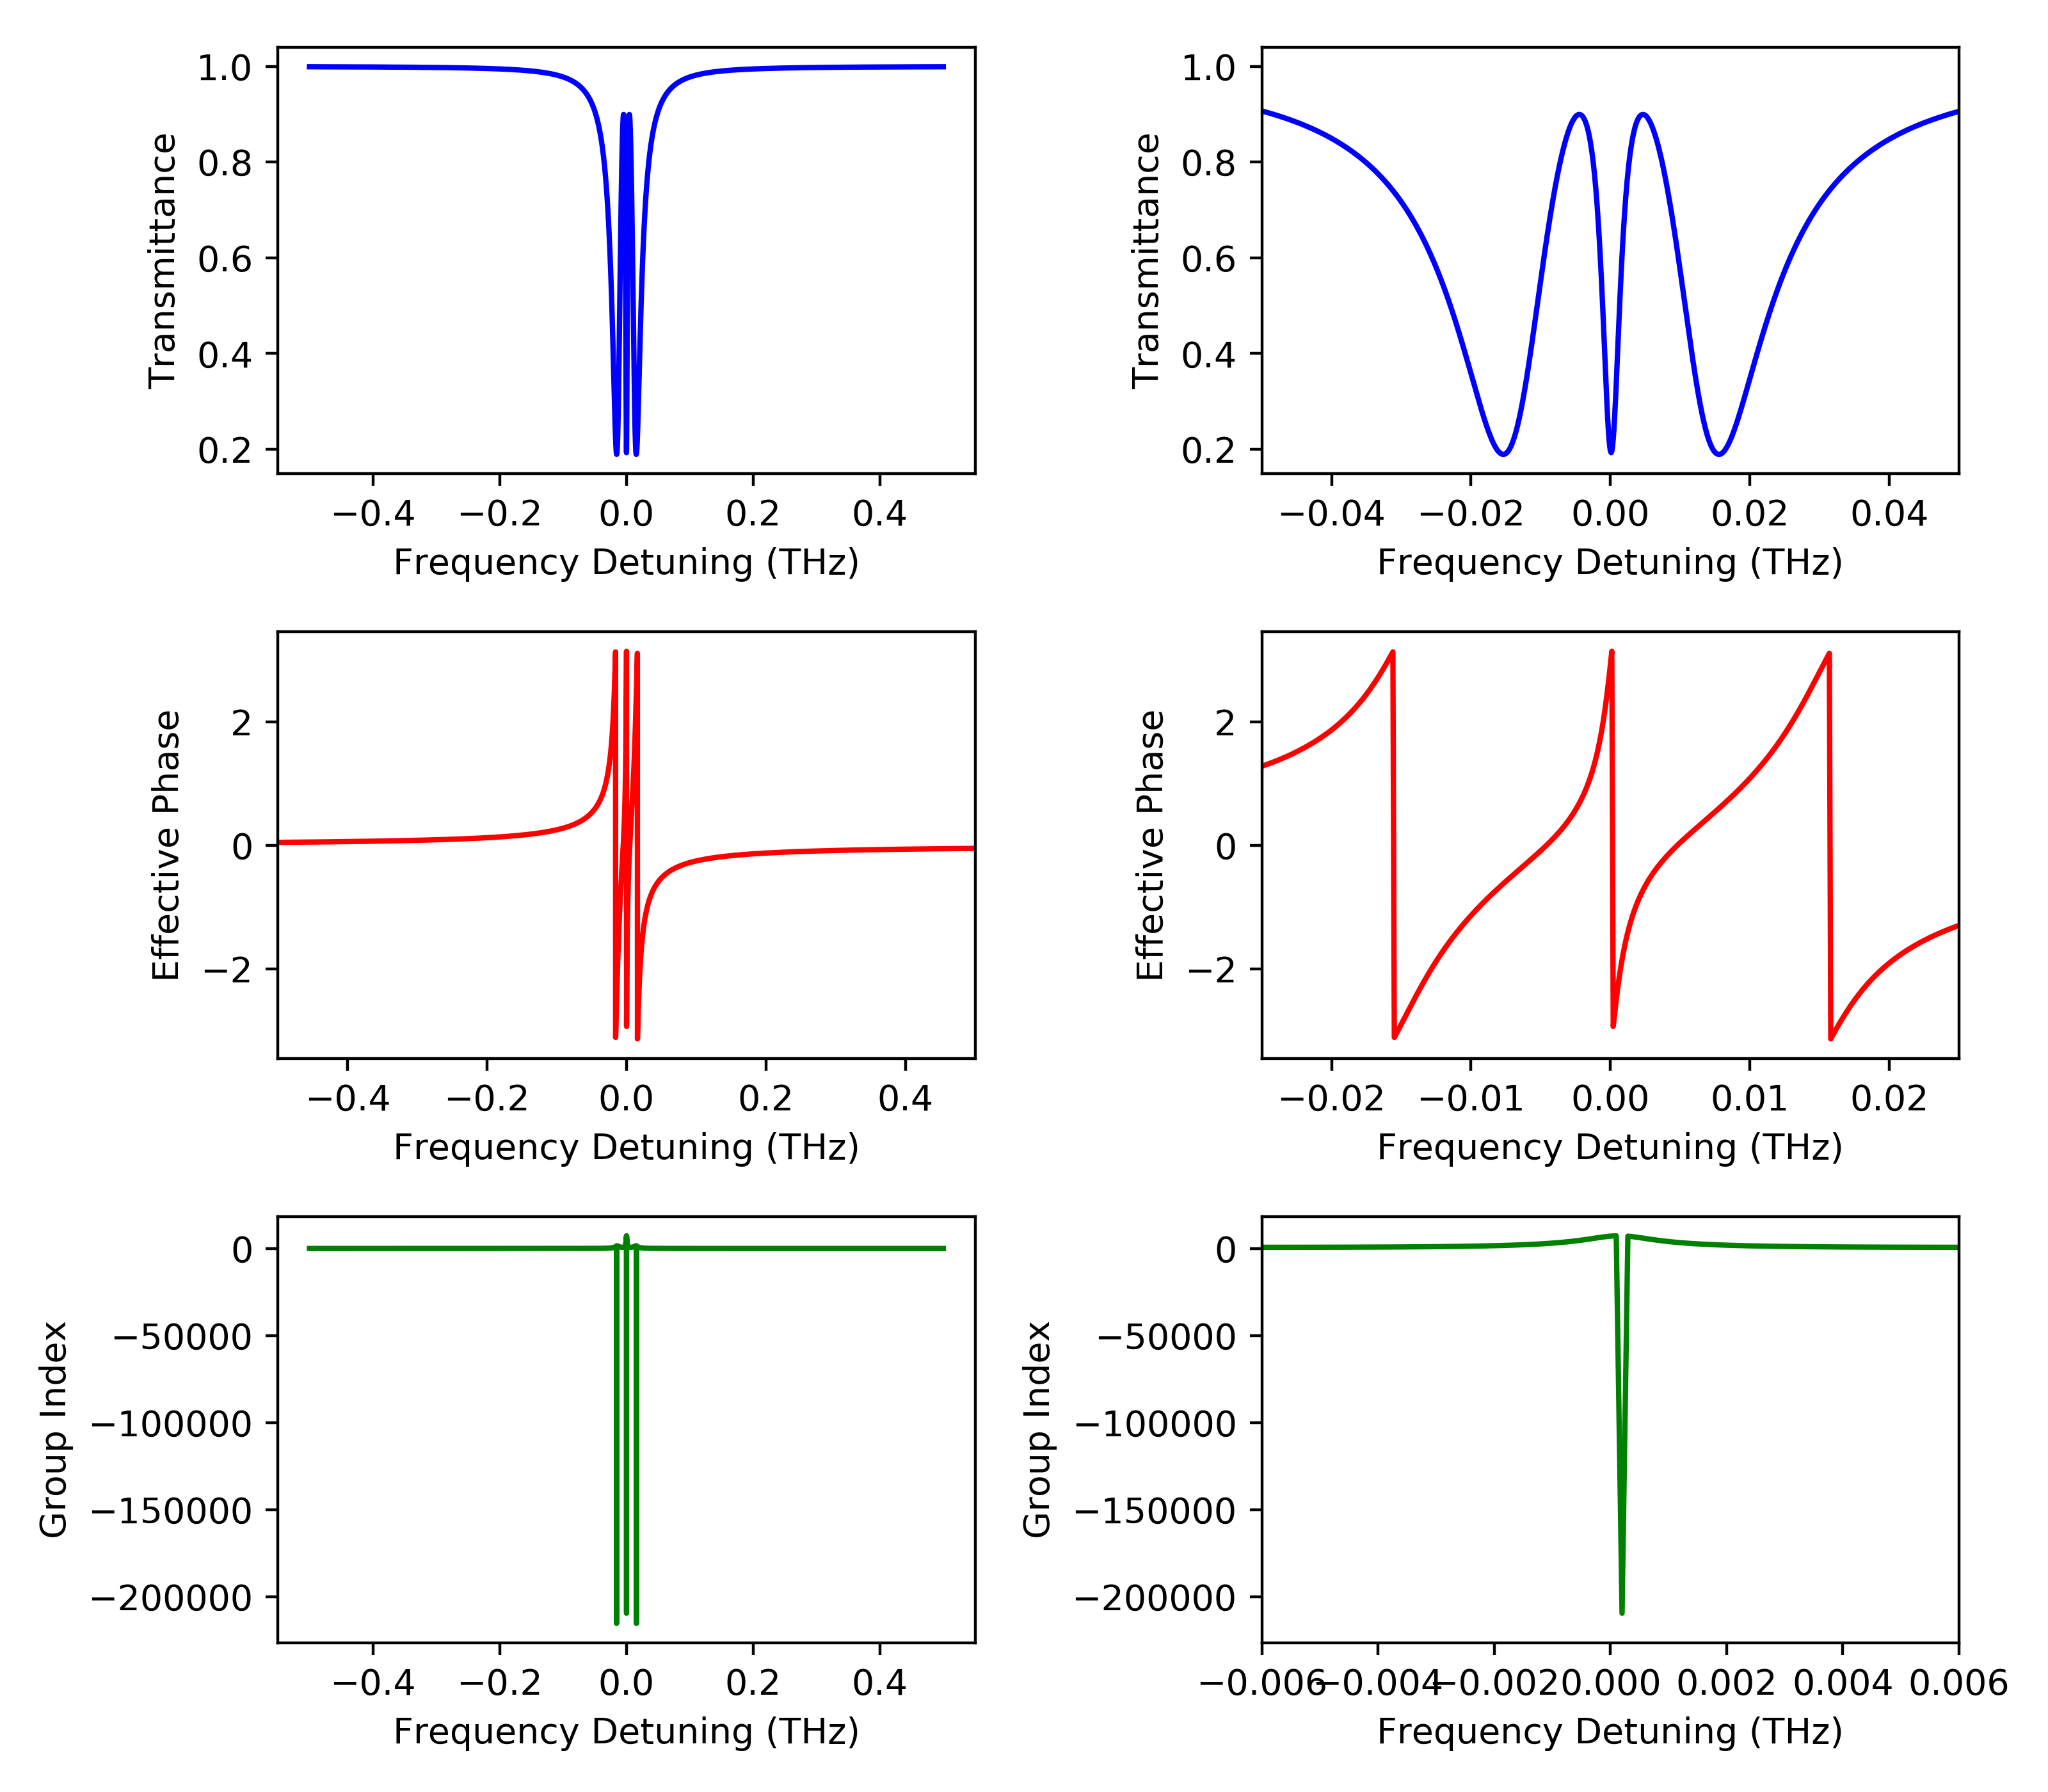
\includegraphics[width=0.90\textwidth]{EIAinEIT.png}
\caption{CRIA observered in an CRIT transmission in three resonator system with its phase in red and group index in green.}
\end{figure}

In Fig. 4.3, we see a CRIT spectrum. When we again zoom into the transmission, we see a narrow dip on resonance. This narrow dip shows us that we actually have a CRIA resonance at the center of a CRIT resonance.

We see that the graph dips to near zero on-resonance but have high transmission values off-resonance. This transmission dip tells us that we can filter out exactly this narrow spectrum of resonant frequencies. 
The phase of the system is shown in red and we see features of superluminal group velocity dispersion. The slope of this graph is negative on resonance.

The group index, shown in green, also displays group index of very high negative value. Its value is $\approx -209493$ meaning superluminal and negative group velocities of resonant frequency.


\subsection{Cascaded CRIA and CRIT in Absorption}
In Fig. 4.4, we will observe that the transmission can be a lot influenced if we were to change the coupling effects between the resonators. The system parameters are given as, $r_{1} = 0.999945$, $r_{2} = 0.999999$, and $r_{3} = 0.999999$. The $\mathcal{Q}-factors$ are $1\times10^{5}, 1\times10^{6}$ and $1\times10^{7}$ for first second and third resonator respectively. This tells us a lot about how our signal is transmitted and how much use can we achieve from the single system by changing a few of its properties. In Fig. 4.3, we change the coupling parameters in all of the resonators and have achieved a rather interesting transmission spectrum.

We can clearly see what looks like an absorption spectrum of a single resonator, has a narrow, actually CRIT peak within the broader CRIA transmission dip (zoomed on the right). This peak also has a dip on resonance due to the resonance of the third resonator. Now we observed cascaded results of CRIT within an absorption and CRIA inside that CRIT. 

The effective phase of the system, at first, also seems like that of a single resonator system but zooming into the graph tells another story. On the right, we can see three distinct features caused by coupling between the three resonators and have a negative slope on resonance. This negative slope refers that superluminal light is achieved the resonance.

The group index plot, shown in green, also displays a negative group index $\approx -38$ on resonance and positive index peaks off resonances. The negative group delay also predicts superluminal velocities of the resonant frequencies.
\newpage
\begin{figure}[h]
\centering
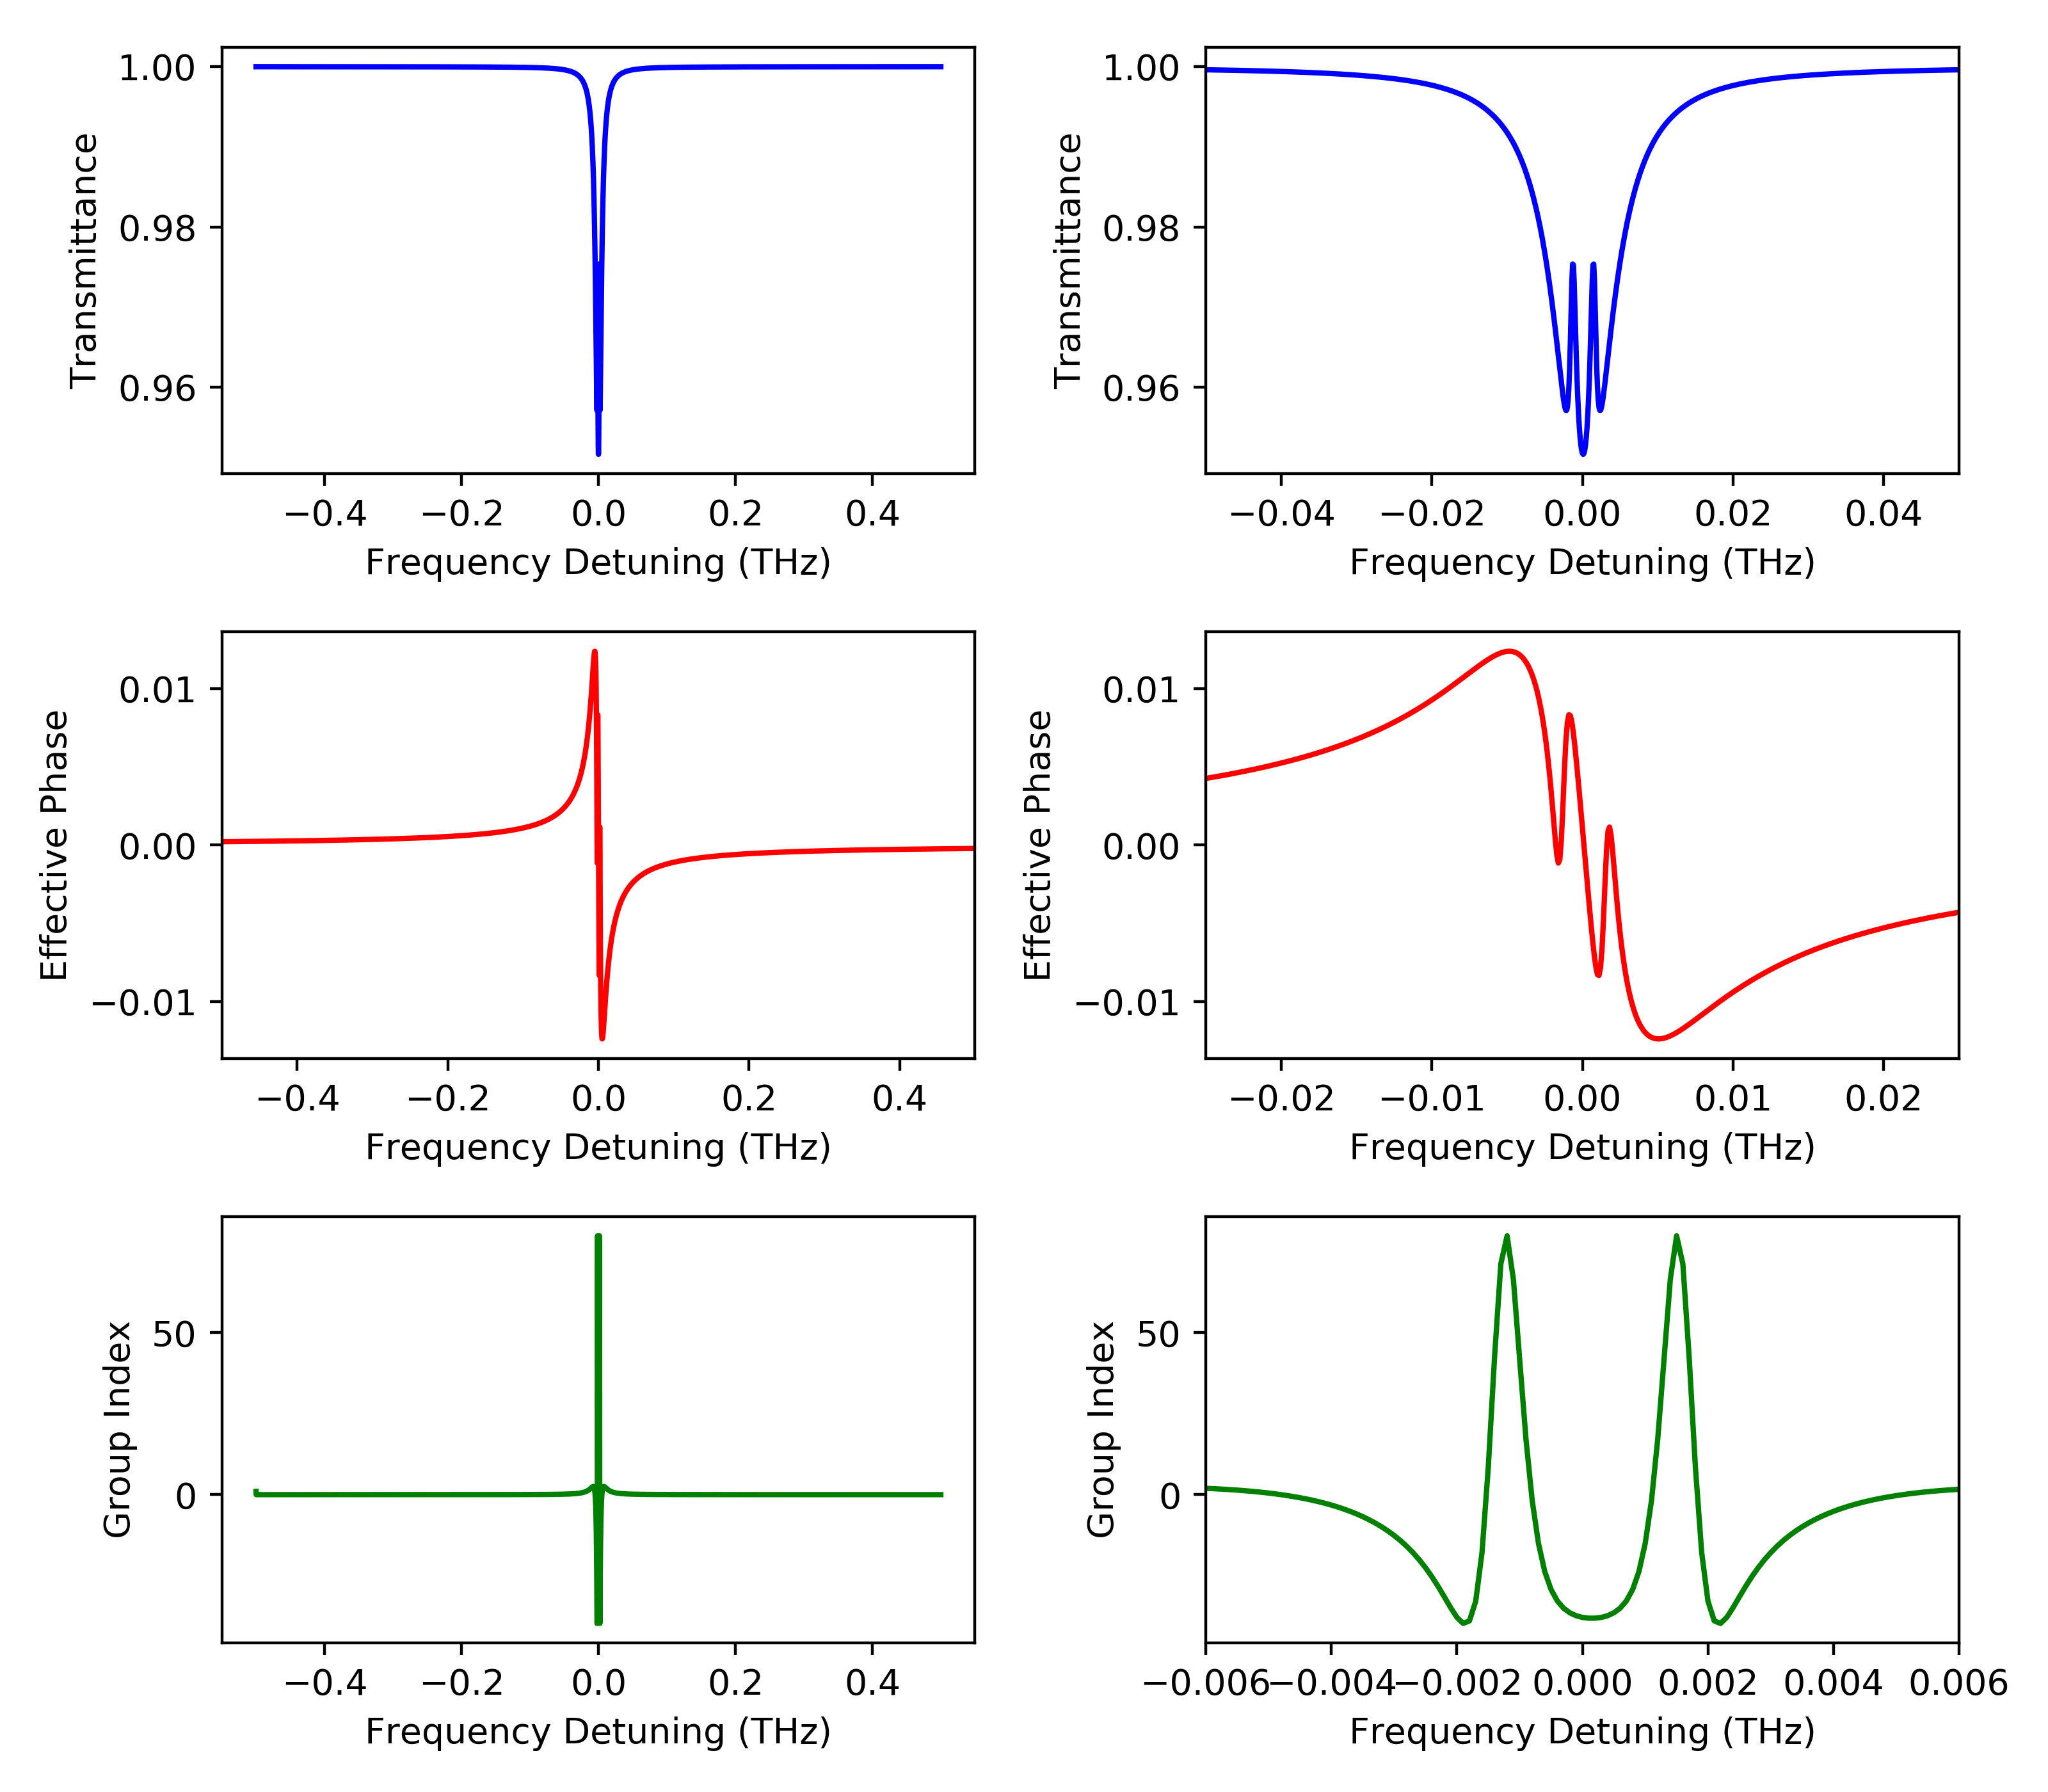
\includegraphics[width=1\textwidth]{EIT_EIA2_all.png}
\caption{Cascaded resonance effects in the three-resonator system with its phase in red and group index in the green. Magnified views of resonances and phase are also given for clear illustration.}
\end{figure}

\subsection{Double CRIA}
We now demonstrate a double CRIA resonance (see Fig. 4.5). This means that two narrow dips are realized within a broader dip. This is in contrast to a typical CRIA where only one narrow dip is present inside a broader dip. This double EIA or CRIA is obtained by slight detuning the system and changing the coupling effects. 


\begin{figure}[t]
\centering
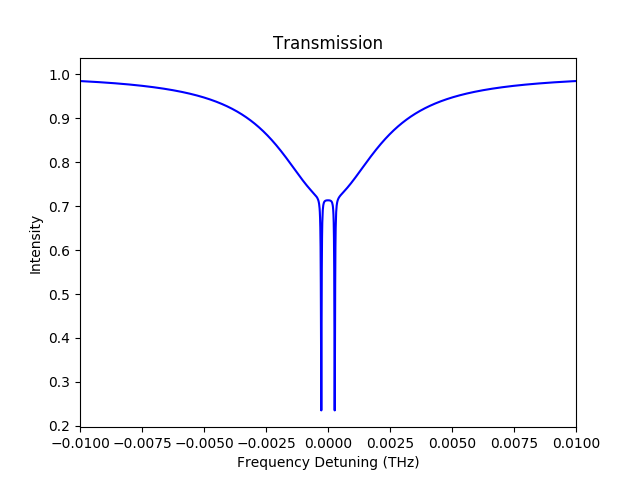
\includegraphics[scale=0.5]{2_EIA.png}
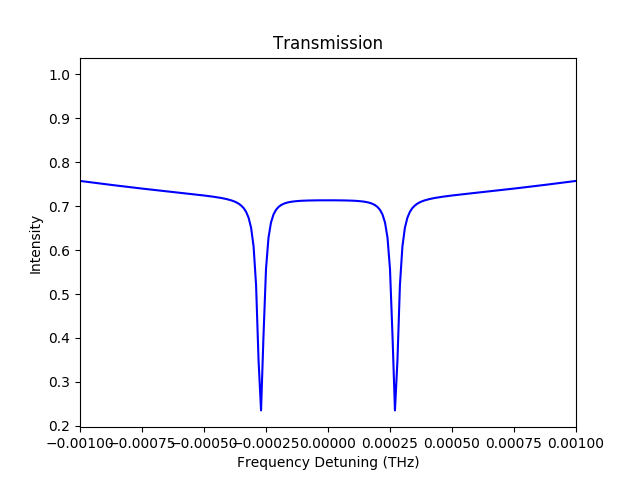
\includegraphics[scale=0.5]{2_EIAa.png}
\caption{Double transmission dips observed inside an EIA like transmission off resonant to the spectrum.}
\end{figure}

In Fig. 4.5 we can clearly see that two narrow peaks, which are caused by the two resonances of the coupled resonators, 2 and 3 respectively. And the broader dip above them is caused by the resonance of the first resonator. 


This allowed us to observe an effect which resembles the CRIA in two resonator system but this time now we have two narrow dips off resonances. This tells us that we have CRIA like properties and transmission have two narrow absorption lines but on the off-resonance. The resonant frequencies will experience very little absorption and will be mostly transmitted. 

The phase and group velocities of this case are not discussed as the purpose of this study were not to discuss the enhanced dispersion. The dispersive properties of these resonances will be similar to the ones discussed above. The true meaning is to show enhanced transmittance.


\subsection{Double CRIT}
We now demonstrate a double CRIT resonance in Fig. 4.6. This means that two narrow peaks are realized within another narrow dip on-resonance. This is in contrast to a typical CRIT where only one narrow peak is present. This double EIT or CRIT is obtained by changing the coupling effects. 

\begin{figure}[t]
\centering
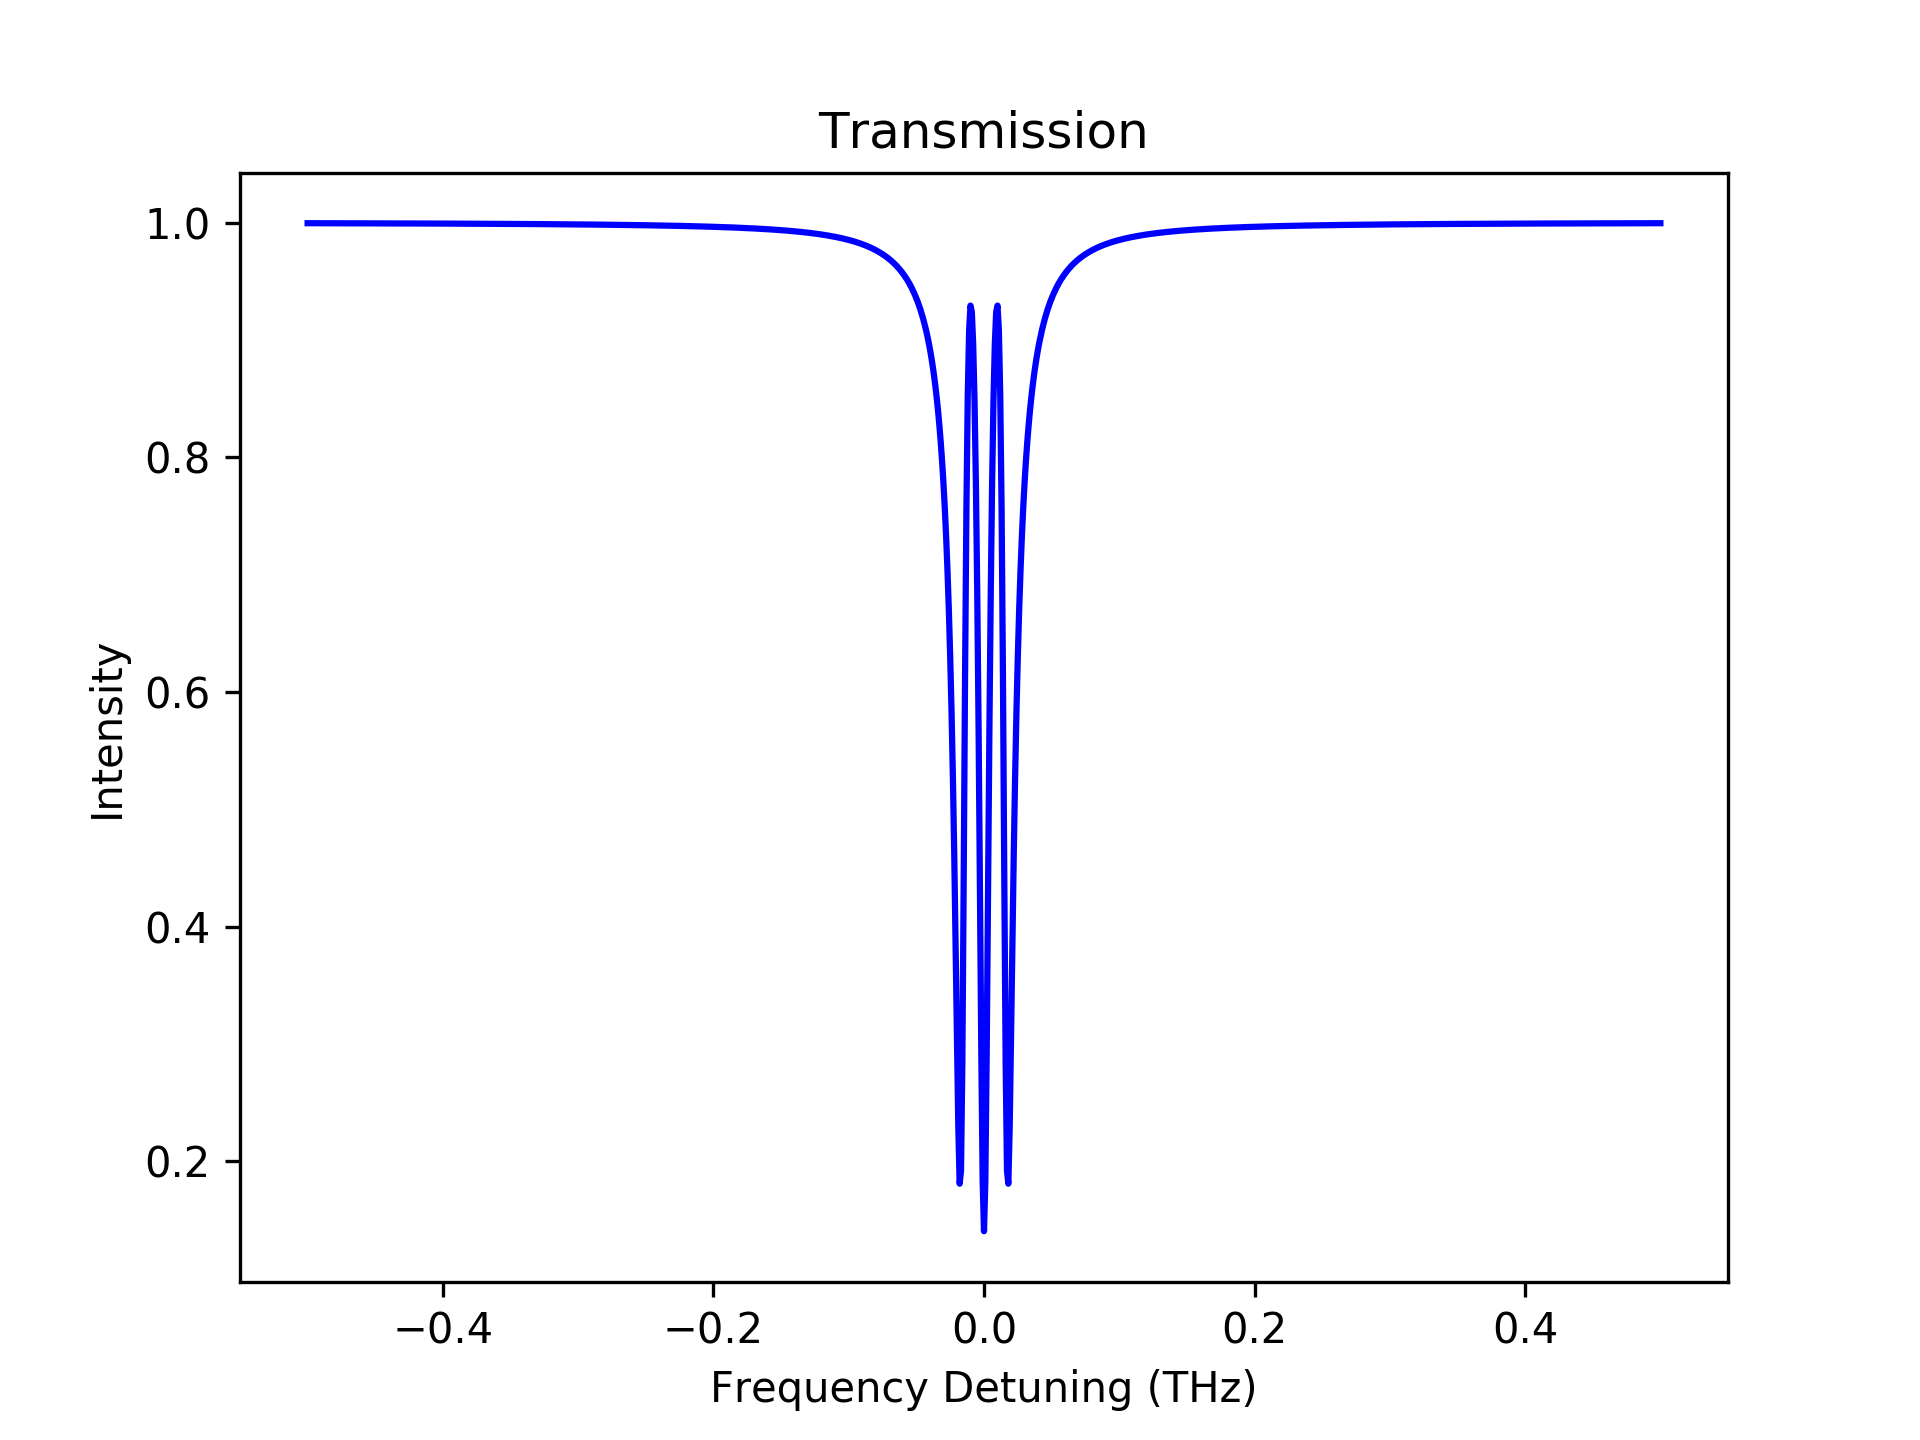
\includegraphics[scale=0.5]{double_EIT.png}
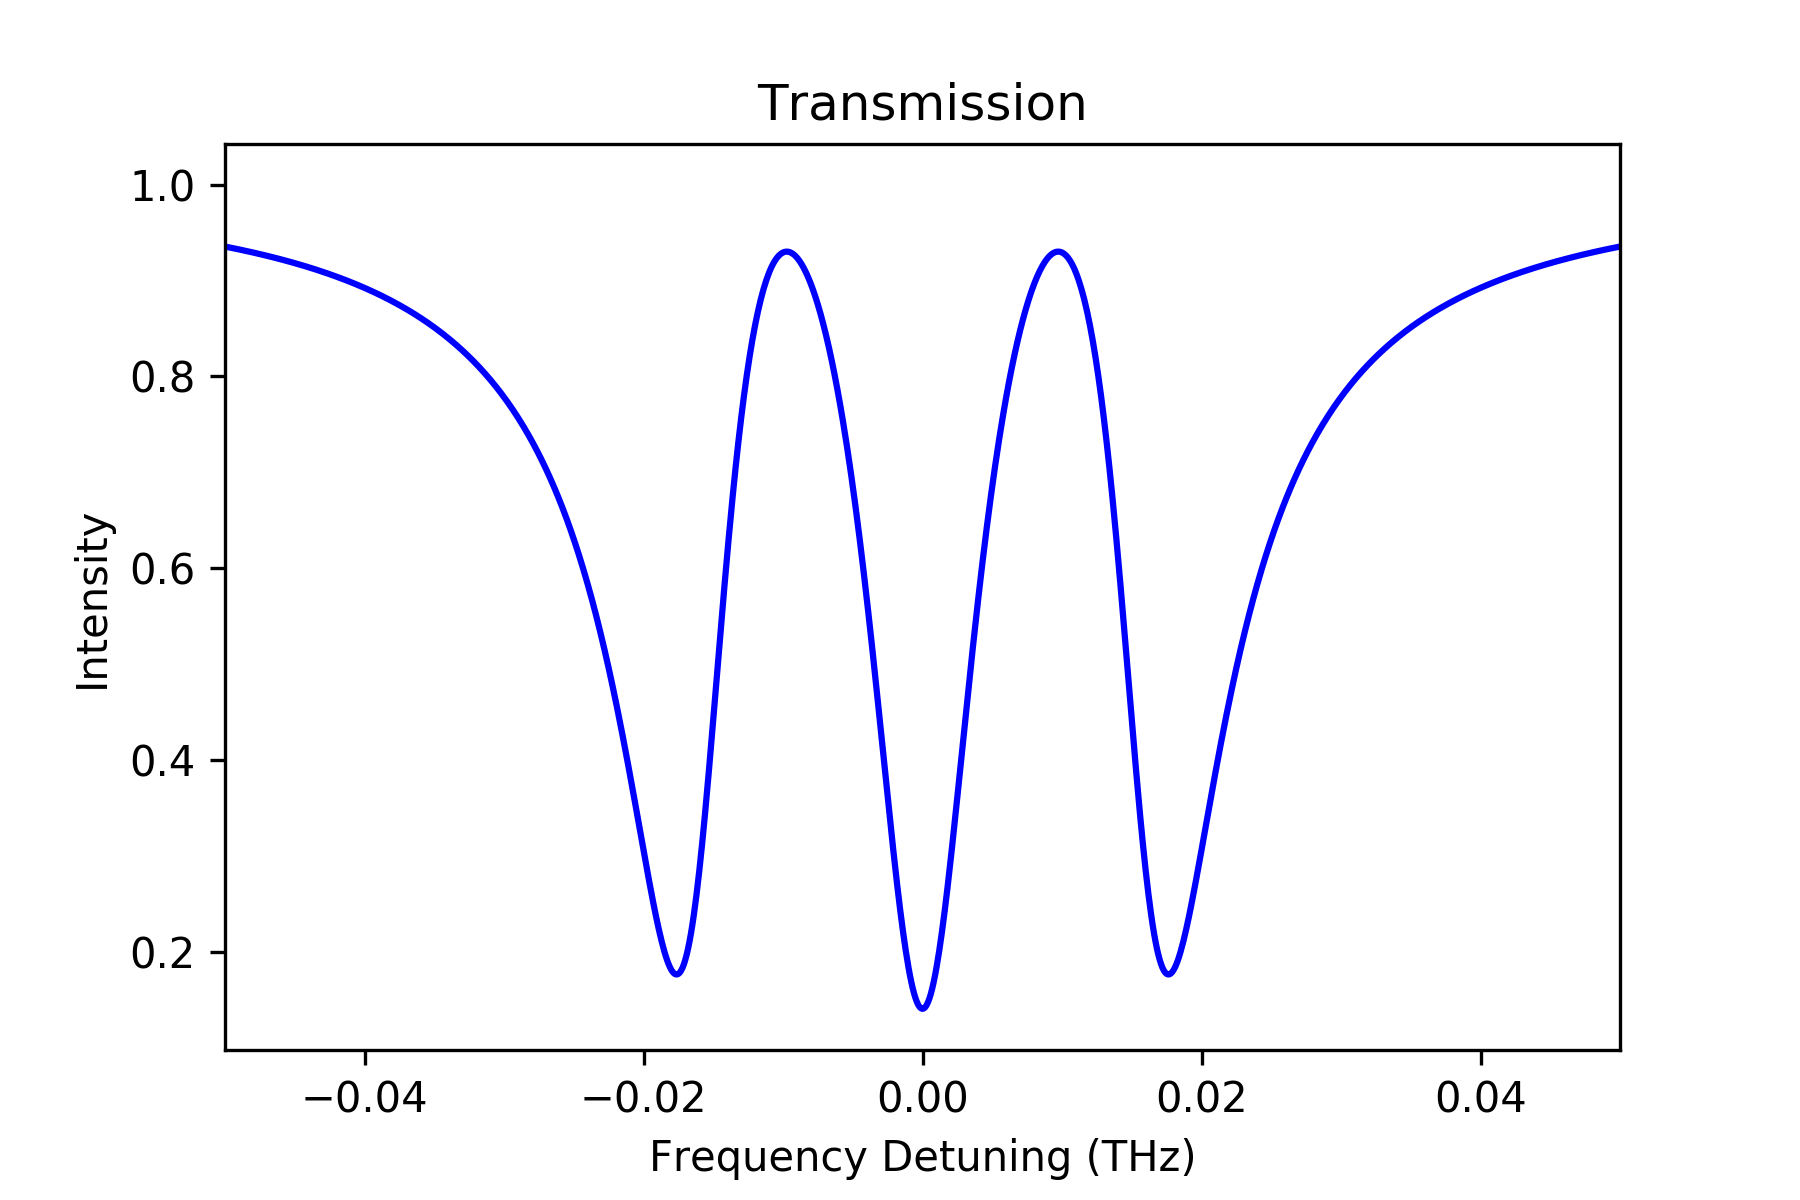
\includegraphics[scale=0.5]{double_EITa.png}
\caption{Double transmission peaks observed inside an EIT like transmission off resonant to the spectrum.}
\end{figure}


From these results, we concluded that increasing the number of resonators in the system and mutually coupling them with each other, enables us to demonstrate the versatility of the cascaded resonances. These resonances can be then utilized and achieved in practical applications to make use of them in important tasks. Optical tunability and signal filtration of specific frequencies can be achieved by using similar systems and having similar effects on them.

\newpage
\section{Discussion}
We have examined the spectral and dispersive properties of a course of three mutually coupled ring resonators. We have discovered various one of a kind cascaded resonances which show particular spectral and dispersive conduct. In view of our request, we propose new uses of coupled resonators for future quantum and optical information and communication technologies. Interacting triple cavities were previously investigated using one and two-dimensional photonic crystals for parametric oscillations [5] and group delay control [6], respectively. Furthermore, double anti-crossing behavior was recently demonstrated using triple microtoroid cavities [7]. Tunable slow and fast light in triple one-dimensional photonic crystal microcavities has also been demonstrated owing to the tuning of the resonant wavelength.

\newpage
\section*{References}
\addcontentsline{toc}{section}{References}

\paragraph{\normalfont \large $[1]$ S. H. Autler and C. H. Townes, “Stark effect in rapidly varying fields,” Phys. Rev. \textbf{100} (1955). \\ 
\\$[2]$ S. E. Harris, "Electromagnetically Induced Transparency" Physics Today, July 1997. \\
\\$[3]$ D. D. Smith, H. Chang, K. A. Fuller, A. T. Rosenberger, and R. W. Boyd, “Coupled-resonator-induced transparency,” Phys. Rev. A \textbf{69}, 063804 (2004). \\
\\$[4]$  A. Naweed, G. Farca, S. Shopova, and A. T. Rosenberger, “Induced transparency and absorption in coupled
whispering-gallery microresonators,” Phys. Rev. A \textbf{71} (2005).\\
\\$[5]$ C. Diederichs, J. Tignon, G. Dasbach, C. Ciuti, A. Lemaître, J. Bloch, P. Roussignol, and C. Delalande, “Parametric oscillation in vertical triple microcavities,” Nature \textbf{440}, 904 (2006).\\
\\$[6]$ D. O’Brien, A. Gomez-Iglesias, M. D. Settle, A. Michaeli, M. Salib, and T. F. Krauss, “Tunable optical delay using photonic crystal heterostructure nanocavities,” Appl. Phys. Rev. B \textbf{76}, 115110 (2007).\\
\\$[7]$ C. Yang,  X. Jiang Q. Hua, S. Hua, Y. Chen, and M. Xiao, “Realization of controllable photonic molecule based on three ultrahigh-Q microtoroid cavities,” Laser Photonics Rev. \textbf{11} (2007).\\
\\$[8]$ A. Naweed (to be published).}